\documentclass[tikz]{standalone}
\begin{document}
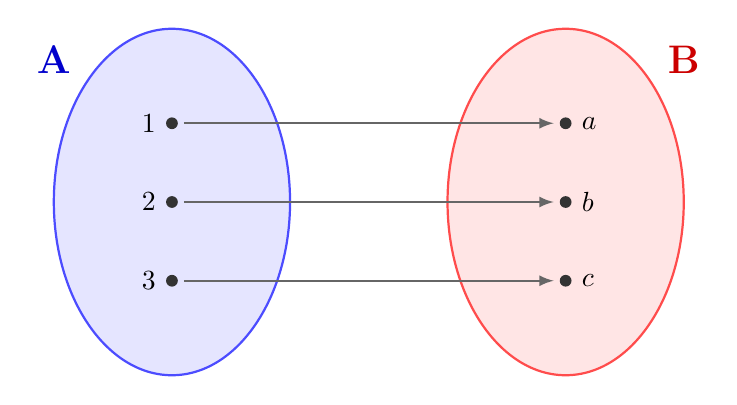
\begin{tikzpicture}[>=latex]

% --- Global TikZ Styles for Consistency ---
\tikzset{
    setA/.style={fill=blue!10, draw=blue!70, thick},
    setB/.style={fill=red!10, draw=red!70, thick},
    labelA/.style={text=blue!80!black, font=\Large\bfseries},
    labelB/.style={text=red!80!black, font=\Large\bfseries},
    point/.style={circle, fill=black!80, inner sep=1.5pt},
    arrow/.style={->, >=latex, thick, draw=black!60, shorten >=2pt, shorten <=2pt}
}

    % Verzameling A
    \path[setA] (0, 1.0) ellipse (1.5cm and 2.2cm);
    \node[labelA] at (-1.5, 2.8) {A};
    \node[point, label=left:$1$] (a1) at (0, 2.0) {};
    \node[point, label=left:$2$] (a2) at (0, 1.0) {};
    \node[point, label=left:$3$] (a3) at (0, 0.0) {};

    % Verzameling B
    \path[setB] (5, 1.0) ellipse (1.5cm and 2.2cm);
    \node[labelB] at (6.5, 2.8) {B};
    \node[point, label=right:$a$] (b1) at (5, 2.0) {};
    \node[point, label=right:$b$] (b2) at (5, 1.0) {};
    \node[point, label=right:$c$] (b3) at (5, 0.0) {};

    \draw[arrow] (a1.east) -- (b1.west);
    \draw[arrow] (a2.east) -- (b2.west);
    \draw[arrow] (a3.east) -- (b3.west);
    
\end{tikzpicture}
    
\end{document}